\newcommand{\figureButtonBounceGraph}[1]{
  \def\lang{\detokenize{#1}}
  \def\langRu{\detokenize{ru}}
  \def\langEn{\detokenize{en}}
  \def\figureCaption{XXX: No translation.}
  %% \def\figureUnit{$\mu\mbox{s}$}
  \ifx \lang\langRu
  \def\figureCaption{
    Эффект ``дребезга'' контактов.
  }
  \fi
  \ifx \lang\langEn
  \def\figureCaption{
    Button bounce effect.
  }
  \fi
  \begin{figure}[H]
    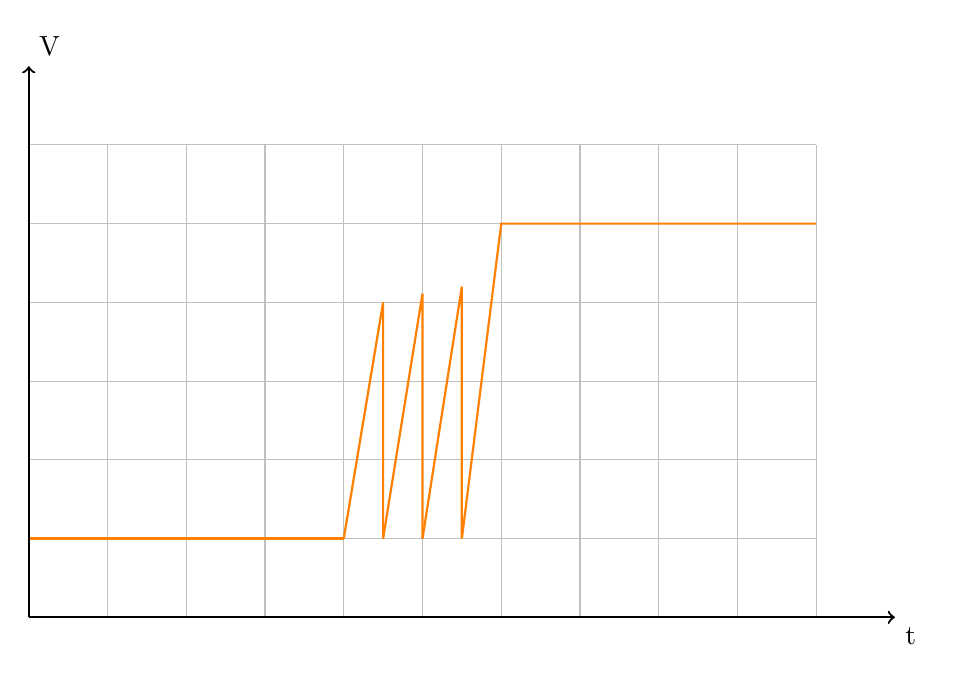
\begin{tikzpicture}[samples=200, domain=0:5*360]
      \draw[lightgray] (0, 0) grid (10, 6);
      \draw[thick, orange] (0,  1) -- (4,   1);
      \foreach \x in {4.0, 4.5, 5.0} {
        \pgfmathsetmacro{\mx}{\x + 0.25 + random(0,2) / 8}
        \pgfmathsetmacro{\my}{5 - random(0,4) / \x}
        \pgfmathsetmacro{\ex}{\x + 0.5}
        \draw[thick, orange] (\x,  1)
        -- (\mx, \my)
        -- (\ex, 1);
      };
      \draw[thick, orange] (5.5, 1) -- (6,  5) -- (10, 5);
      \draw[thick, ->] (0, 0) -- (11, 0) node[anchor=north west] {t};
      \draw[thick, ->] (0, 0) -- (0,  7) node[anchor=south west] {V};
    \end{tikzpicture}
    \caption{\figureCaption}
    \label{fig:button-bounce-graph}
  \end{figure}
}
